\documentclass{article}
\usepackage{calc}
\usepackage{graphicx}
\usepackage{float}
\usepackage{eso-pic}

\usepackage{array}    % For better column alignment
\usepackage{longtable} % For tables that span multiple pages
\usepackage{setspace}   % For adjusting line spacing
\usepackage{booktabs}   % For better looking tables (optional)
\usepackage{makecell}   % For custom cell formatting, especially for headings
\usepackage{hyperref}

\usepackage{ulem}
\usepackage{amsmath}\
\usepackage[a4paper, margin=1 in]{geometry}


\newlength{\PageFrameTopMargin}
\newlength{\PageFrameBottomMargin}
\newlength{\PageFrameLeftMargin}
\newlength{\PageFrameRightMargin}

\setlength{\PageFrameTopMargin}{0.8cm}
\setlength{\PageFrameBottomMargin}{0.8cm}
\setlength{\PageFrameLeftMargin}{0.8cm}
\setlength{\PageFrameRightMargin}{0.8cm}

% Increase padding inside cells
\renewcommand\arraystretch{2} % Increase row height
\setlength{\tabcolsep}{12pt}    % Increase horizontal padding (space between text and cell border)

\makeatletter

\newlength{\Page@FrameHeight}
\newlength{\Page@FrameWidth}

\AddToShipoutPicture{
  \thinlines
  \setlength{\Page@FrameHeight}{\paperheight-\PageFrameTopMargin-\PageFrameBottomMargin}
  \setlength{\Page@FrameWidth}{\paperwidth-\PageFrameLeftMargin-\PageFrameRightMargin}
  \put(\strip@pt\PageFrameLeftMargin,\strip@pt\PageFrameTopMargin){
    \framebox(\strip@pt\Page@FrameWidth, \strip@pt\Page@FrameHeight){}}}

\makeatother

\begin{document}

\begin{center}
    \Huge \underline{Lab Notebook}
\end{center}
    \vspace{1em}

    \begin{center}
    {\Large
    \underline{Software Tools and Technology Lab}} 
    \end{center}

    \vspace{0.4em}
    
    \begin{center}
        {\Large \underline{SEBCA1191}}
    \end{center}




\begin{figure}[h]
    \centering
    \includegraphics[width=0.75\linewidth]{front.PNG}
    
    \end{figure}

\vspace{1cm}

\begin{center}
    
\setlength{\arrayrulewidth}{0.4mm}
\setlength{\tabcolsep}{20pt}
\renewcommand{\arraystretch}{2}
\begin{tabular}{ |c|c|c| }
\hline
\multicolumn{3}{|c|}{\Large \textbf{\textit{Group 24}}} \\
\hline
NAME & ROLL NO.& DEPARTMENT \\
\hline
Snehal Das [Leader] & 30001223015 & BCA \\
Nupur Sinha & 30001223002 & BCA \\
Nikita Debnath & 30001223023 & BCA \\
Swastik Das & 30001223075 & BCA \\
Sunit Modak & 30084323005 & BSc in Data Science \\

\hline
\end{tabular}
\end{center}

\newpage

\begin{center}
    \Huge{\textit{\textbf{Index Page}}}

\vspace{1.1cm}
\end{center}


% Define the table with width 80% of textwidth
\begin{center}
    
\large \begin{longtable}{|p{0.08\textwidth}|p{0.13\textwidth}|p{0.45\textwidth}|p{0.145\textwidth}|}
    \hline
    \textbf{\Large S.No.} & \textbf{\Large Subject} & \textbf{\Large Description} & \textbf{\Large Pages} \\
    \hline
    \endfirsthead
    \hline
    \textbf{\Large S.No.} & \textbf{\Large Subject} & \textbf{\Large Description} & \textbf{\Large Pages} \\
    \hline
    \endhead
    \hline
    1 & Calculator & Download GitHub desktop in your system, create a local repository. Build a C programme of calculator in the local repository, commit and publish it as a public repository. & 3-4 \\
    \hline
    2 & Matrices & How to create matrices of different types in LaTeX: bmatrix, pmatrix, vmatrix,Vmatrix & 5-8 \\
    \hline
    3 & CV using LaTeX & Your task is to create your CV using LaTeX documen & 8-9 \\
    \hline
    4 & Mathematical Document & Your task is to create your LaTeX document. 
    The document should be formatted to look exactly like an attachment. & 9-10 \\
    \hline
    5 & Git Branching and Merging & A hands-on task to understand and implement Branching, Merging, conflict resolution in Git. & 11-12 \\
    \hline
    
    
\end{longtable}
\end{center}
\newpage

\begin{center}
    \Huge I. \underline{Calculator Repository}
    \end{center}
    \vspace{1em}

    \begin{center}
        \Large GitHub Desktop
    \end{center}

    \vspace{0.4em}
    
    \begin{center}
        \large By Snehal Das
    \end{center}


\section{\underline{Description:}}
The task was divided into two parts: \vspace{0.2cm}\newline

1. Download GitHub desktop in your system (https://desktop.github.com/download/) and go through the tutorial for private repository publish. \vspace{0.2cm}
\newline

2. Create a local repository. Build a C programme of calculator in the local repository, commit and publish it as a public repository. \vspace{0.2cm}
\newline

\section{\underline{Steps:}}
The task was achieved by following the below mentioned steps:-
\newline

1. Download the GitHub Desktop Application through the given link. Then basic account setup. \vspace{0.5cm}

2. Using the OPEN IN SUBMILE TEXT (whichever text editor you have) option, update README file. Come back to app, and commit the change, using meaningful message. \vspace{0.5cm}

3. In your Desktop Application, go to file --> New Repository --> Give Name, Description, and specify local path. Check or uncheck README file and --> Create Repository \vspace{0.5cm}

4. In text editor, create a C file called basicCalculator, and write your code, save. Using similar steps, commit the change. \vspace{0.5cm}

5. Now Publish Repository, to push the repo into remote Git server. \vspace{0.5cm}

\newpage
\subsection{\underline{Code Snippet:}}

\begin{figure}[h!]
    \centering
    \includegraphics[width=0.7\textwidth]{calculator1.PNG}
    \caption{Source Code}
\end{figure}

\centering

\large This is a simple Calculator program in C, which takes in 3 inputs from the user- the two operands, and the operator. The program makes use of the SWITCH CASE statement to implement conditions, calculating and displaying the result accordingly.

\vspace{1.3cm}

\begin{figure}[h!]
    \centering
    \includegraphics[width=0.7\textwidth]{calculator2.PNG}
    \caption{Output}
\end{figure}

\newpage

\begin{center}
    \LARGE{\textbf{2. \underline{How to create Matrix in LaTeX}}}
\end{center}
\vspace{0.2cm}
 \begin{center}
     \section*{\underline{Lab Assignment by Nupur Sinha}}
\end{center}
\LARGE{To create a matrix in LaTeX, we use the \texttt{\textbf{amsmath}} package, which provides various environments for displaying matrices. Here’s a basic guide on how to create a matrix and the different options available:}
\vspace{0.1cm}
\begin{center}
\begin{itemize}
    \item{\underline{\textbf{Include the \texttt{amsmath} Package}}}
\end{itemize} 
\end{center}
First, ensure you have the \texttt{amsmath} package included in your LaTeX document preamble. Add the following line:
\begin{verbatim}
\usepackage{amsmath}
\end{verbatim}
\begin{center}
    \begin{itemize}
        \item {\textbf{\underline{Matrix Environments}}}
    \end{itemize}
\end{center}
\LARGE{
There are several environments for creating matrices, depending on how you want them formatted. Here are the most common ones:}

\begin{itemize}
  \item \texttt{matrix}: A basic matrix without brackets.
  \item \texttt{bmatrix}: A matrix with square brackets.
  \item \texttt{pmatrix}: A matrix with parentheses.
  \item \texttt{vmatrix}: A matrix with vertical bars.
  \item \texttt{Vmatrix}: A matrix with double vertical bars.
\end{itemize}
\begin{center}
        \item {\textbf{\underline{\LARGE{Syntax}}}}
\end{center}

\LARGE{The syntax for creating a matrix is similar across different environments. Use the \texttt{\textbackslash begin\{environment\}} and \texttt{\textbackslash end\{environment\}} commands to enclose the matrix content. Separate the elements in each row with \texttt{\&} and 

end each row with \texttt{\\}.

Here’s an example of a 2x2 matrix in each environment:}
\begin{verbatim}
[ 
$ \begin{matrix}
    1 & 0 \\
    0 & 1 
\end{matrix}
$ ]

\begin{bmatrix}   [
 $   \begin{matrix}
    1 & 0\\
    0 & 1
    \end{matrix}
 $   ]

a_{11} & a_{12} \\
a_{21} & a_{22}
\end{bmatrix}

\begin{pmatrix}
a_{11} & a_{12} \\
a_{21} & a_{22}
\end{pmatrix}

\begin{vmatrix}
a_{11} & a_{12} \\
a_{21} & a_{22}
\end{vmatrix}

\begin{Vmatrix}
a_{11} & a_{12} \\
a_{21} & a_{22}
\end{Vmatrix}
\end{verbatim}

\begin{center}
\section*{\textbf{\underline{\LARGE{Explanation}}}}
\end{center}
\begin{itemize}
  \item \texttt{\textbackslash begin\{matrix\} ... \textbackslash end\{matrix\}}: Creates a matrix with no surrounding brackets.
  \item \texttt{\textbackslash begin\{bmatrix\} ... \textbackslash end\{bmatrix\}}: Surrounds the matrix with square brackets.
  \item \texttt{\textbackslash begin\{pmatrix\} ... \textbackslash end\{pmatrix\}}: Surrounds the matrix with parentheses.
  \item \texttt{\textbackslash begin\{vmatrix\} ... \textbackslash end\{vmatrix\}}: Surrounds the matrix with single vertical bars, often used to denote determinants.
  \item \texttt{\textbackslash begin\{Vmatrix\} ... \textbackslash end\{Vmatrix\}}: Surrounds the matrix with double vertical bars, also used for determinants or norms.
\end{itemize}


\newgeometry{top=1 in}
\begin{normalsize}
    

\section{\centering{\uline{My LATEX Document and Mathematical Notation}}}
    \vspace{.5cm}
    \centerline{LATEX File}
    \vspace{.5cm}
    \centerline{Nikita Debnath}
    \vspace{.5cm}
    \subsection{\uline{Description:}}
    \begin{enumerate}
        \item At first we have to create a overleaf account.
        \item Then create a new blank file and the write down the code.
    \end{enumerate}

    
    \subsection{\uline{Steps:}}
    \begin{enumerate}
    \item \textbf{Basic LaTeX Document Structure:}
    \\
    Every LaTeX document starts with \verb|{\begin{document}| and ends with \verb|{\end{document}|. This structure defines how the document will be formatted and organized.

    \item \textbf{Document Type, Title, Author, and Photo Integration:}  
    \\ 
    To define the type of the document, we have to use \verb|\documentclass{article}|. Use the \verb|\title|, \verb|\author|, and \verb|\date| commands to display document metadata. Insert photos using the graphicx package and \verb|\includegraphics{image_file_name.jpg}| command.
    \begin{enumerate}
    \item Input:
    \begin{verbatim}
        \documentclass{article}
        \usepackage{graphicx} 
        \title{My First LATEX Doucument}
        \date{\today}
        \author{Nikita Debnath}
        \date{September 2024}
        \begin{document}
        \maketitle
        \begin{center}
        
\includegraphics[width=0.3\textwidth]{n.jpg}   
        \end{center}
        \end{document}
    \end{verbatim}
    \item Output :
    \begin{flushleft}
        \includegraphics[width=0.3\textwidth]{basic_sturcture.png}
    \end{flushleft}         
    \end{enumerate}

    \item \textbf{Formatting and Bulleted Lists:}
    \\
    LaTeX offers various environments like itemize and enumerate for lists, and basic text can be formatted into sections and subsections with proper headers.
    \begin{enumerate}
        \item \textbf{Section :}
        \\
        The \verb|\section{}| command creates a new section. Sections are the highest-level divisions within a document (after chapters if you're using a book class). It is usually numbered and serves as a top-level heading.
        \begin{enumerate}
            \item \textbf{Syntax:}
            \begin{verbatim}
                \section{Introcuction}
                This is the start of a new section.
            \end{verbatim}
        \end{enumerate}
        \item \textbf{Subsection:}
        \\
        A \verb|\subsection{}|is a sub-division of a section. It creates a smaller heading under the main section.
        \begin{enumerate}
            \item \textbf{Syntax:}
            \begin{verbatim}
                \subsection{sub section}
                This is a subsection within the "Introduction"section.
            \end{verbatim}
        \end{enumerate}
        \item \textbf{Sub-subsection:} 
        \\
        A \verb|\subsubsection{}| is a further subdivision of a subsection. It is used when you need more detailed hierarchical organization.
        \begin{enumerate}
            \item \textbf{Syntax:}
            \begin{verbatim}
                \subsubsection{Background}
                 This is a subsubsection under the "Subsection" subsection.
            \end{verbatim}
        \end{enumerate}
        \item \textbf{Bullet List:}
        \\
        LaTeX uses the itemize environment to create unordered (bullet) lists.
        \begin{enumerate}
            \item \textbf{Syntax:}
            \begin{verbatim}
                \begin{itemize}
                \item First bullet point
                \item Second bullet point
                \item Third bullet point
                \end{itemize}
            \end{verbatim}
        \end{enumerate}
        This will produce a bullet list with three items.
        \item \textbf{Syntax:}
        \\
        \begin{verbatim}
            documentclass{article}
            \begin{document}
            \section{Introduction}
            This is the introduction section.
            \subsection{Motivation}
            This subsection explains the motivation.
            \subsubsection{Background}
            Here is the background information.
            \section{Conclusion}
            Here is a bullet list summarizing key points:
            \begin{itemize}
                \item Point one
                \item Point two
                \item Point three
            \end{itemize}
            \end{document}
        \end{verbatim}
        \item \textbf{Output:}
        \begin{flushleft}
        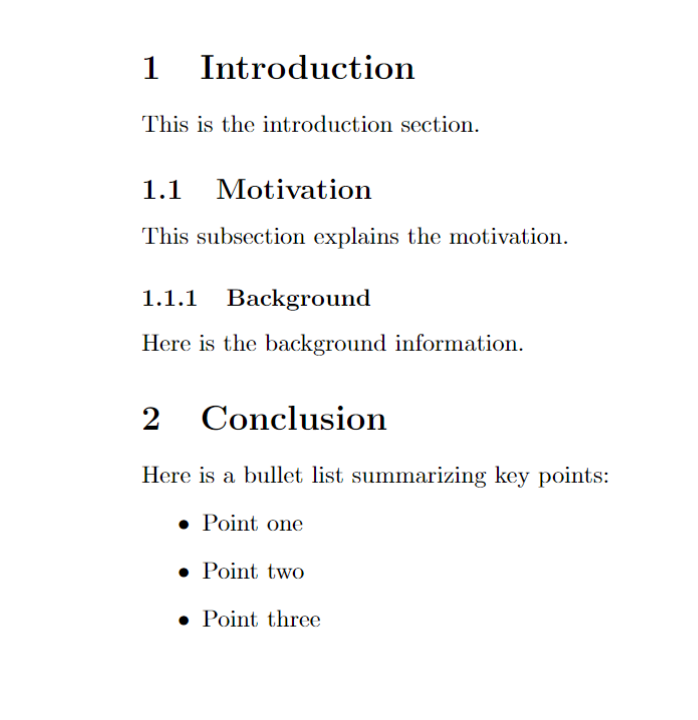
\includegraphics[width=0.4\textwidth]{subsection-bullet.png}
    \end{flushleft}  
    \end{enumerate}
    
    \item Mathematical Expressions, Superscripts, Subscripts, and Greek Letters: 
    LaTeX excels at typesetting mathematical symbols using \verb|\usepackage{amsmath}| or inline display math mode with commands like \verb|$a^b$| for superscripts and \verb|$x_i$| for subscripts.
    \begin{enumerate}
        \item \textbf{Subscript:}
        \\
        Subscripts are used to write smaller text or numbers below the main text.Its writes by underscore.
        \begin{enumerate}
            \item \textbf{Syntax:}
            \begin{verbatim}
                $x_i$
            \end{verbatim}
            \item \textbf{Output:}
            \\
            $x_i$
        \end{enumerate}
        
        \item \textbf{Superscripts:}
        \\
        Superscripts are used to write text or numbers above the main text (for powers or exponents).
        \begin{enumerate}
            \item \textbf{Syntax:}
            \begin{verbatim}
                $x^i$
            \end{verbatim}
            \item \textbf{Output:}
            \\
            $x^i$
        \end{enumerate}

       \item \textbf{Equation Environment:}
        \\
        \begin{enumerate}
        \item The equation environment is used for displaying equations that are centered and automatically numbered.
  
            \begin{enumerate}
                \item \textbf{Syntax:}
            \begin{verbatim}
                \begin{equation}
                    x = 1
                \end{equation}
            \end{verbatim}
            \item \textbf{Output:}
            \\
            \begin{equation}
                    x = 1
            \end{equation}  
            \end{enumerate}
            
        \item This will display the equation  and number it.If you want to avoid numbering the equation, use the syntax -
        \begin{enumerate}
            \item \textbf{Syntax:}
            \begin{verbatim}
                \begin{equation*}
                    x = 1
                \end{equation*}
            \end{verbatim}
            \item \textbf{Output:}
            \\
            \begin{equation*}
                    x = 1
            \end{equation*}
        \end{enumerate}           
        \end{enumerate}
        \item \textbf{Align Environment, Fraction, Square-root:}
        \\
        \begin{enumerate}
        \item The align environment is used for aligning multiple equations. It allows you to align equations at the \& symbol.
        To create fractions, use the \verb|\frac{numerator}{denominator}| command.You can create square roots using the \verb|\sqrt{}| command. If you want an nth root, use \verb|\sqrt[n]{}|.

  
            \begin{enumerate}
                \item \textbf{Syntax:}
            \begin{verbatim}
                \begin{align}
                x + y &= 5 \\
                g(x) &= \frac{1}{x}\\
                F(x) &= \intˆa_b\frac{1}{3}xˆ3
                y &= \sqrt{a}\\
                z &= \sqrt[n]{a}
                \end{align}
            \end{verbatim}
            \item \textbf{Output:}
            \\
                \begin{align}
                x + y &= 5 \\
                g(x) &= \frac{1}{x}\\
                F(x) &= \int^a_b\frac{1}{3}x^3\\
                y &= \sqrt{a}\\
                z &= \sqrt[n]{a}
                \end{align} 
            \end{enumerate}
            
        \item This will display the equation  and number it.If you want to avoid numbering the equation, use the syntax -
        \begin{enumerate}
            \item \textbf{Syntax:}
            \begin{verbatim}
                \begin{align*}
                x + y &= 5 \\
                g(x) &= \frac{1}{x}\\
                F(x) &= \int^a_b\frac{1}{3}x^3
                y &= \sqrt{a}\\
                z &= \sqrt[n]{a}
                \end{align*}
            \end{verbatim}
            \item \textbf{Output:}
            \\
                \begin{align*}
                x + y &= 5 \\
                 g(x) &= \frac{1}{x}\\
                F(x) &= \int^a_b\frac{1}{3}x^3\\
                y &= \sqrt{a}\\
                z &= \sqrt[n]{a}
                \end{align*}
        \end{enumerate}           
        \end{enumerate}
        
    \item \textbf{Matrix:}
        \\
        To create matrices, you can use the bmatrix (for brackets around the matrix), pmatrix (for parentheses around the matrix), or matrix environment.
        \begin{enumerate}
            \item \textbf{Syntax:}
            \begin{verbatim}
                $\begin{matrix}
                    a & b \\
                    c & d
                \end{matrix}$
                \\
                $\begin{bmatrix}
                a & b \\
                c & d
                \end{bmatrix}$
                \\
                $\begin{pmatrix}
                 a & b \\
                 c & d
                \end{pmatrix}$
            \end{verbatim}
            \item \textbf{Output:}
            \\
                $\begin{matrix}
                    a & b \\
                    c & d
                \end{matrix}$
                \\
                $\begin{bmatrix}
                a & b \\
                c & d
                \end{bmatrix}$
                \\
                $\begin{pmatrix}
                 a & b \\
                 c & d
                \end{pmatrix}$
         \end{enumerate}

    \item \textbf{Table:}
        \\
        Tables can be created using the tabular environment. Here's an example of a simple table:
        \begin{enumerate}
            \item \textbf{Syntax:}
            \begin{verbatim}
                \begin{tabular}{|c|c|}
                \hline
                Element & Value \\
                \hline
                1 & 10 \\
                \hline
                2 & 20 \\
                \hline
                3 & 30 \\
                \hline
                \end{tabular}
            \end{verbatim}
            \item \textbf{Output:}
            \\
             \begin{tabular}{|c|c|}
                \hline
                Element & Value \\
                \hline
                1 & 10 \\
                \hline
                2 & 20 \\
                \hline
                3 & 30 \\
                \hline
                \end{tabular}
        \end{enumerate}

     
        \item \textbf{Trigonometric Functions (sin, cos, tan, theta):}
        \\
        LaTeX provides built-in commands for common trigonometric functions and Greek letters like 
        \begin{enumerate}
            \item \textbf{Syntax:}
            \begin{verbatim}
                $\sin \theta$
                \\
                $\cos \theta$
                \\
                $\tan \theta$
            \end{verbatim}
            \item \textbf{Output:}
            \\
             $\sin \theta$
             \\
             $\cos \theta$
             \\
             $\tan \theta$
        \end{enumerate}



    \end{enumerate}

        
    \end{enumerate}

\end{normalsize}
\restoregeometry


\newpage

\section*{Java Swing Application: SymbolApp}
This document describes the Java Swing application named \texttt{SymbolApp}. The application showcases a simple "mind-reading" trick by displaying a grid of symbols and revealing a selected symbol based on user interaction. This document is formatted using LaTeX to provide a clear and professional presentation for academic purposes.

\section*{ 1. Clone the Repository}
At first, I used GitHub Desktop to clone the repository: https://github.com/GeekAyan/STT.
Then I Opened GitHub Desktop, clicked on "File" then "Clone Repository", pasted the URL, and selected my local directory.

\section*{  2. Set Up the Project}
I opened the project in VSCode.
Then Followed the detailed run instructions provided in the README.md file to set up any necessary dependencies and configurations. This could involve installing Python packages or setting environment variables.

\section*{ 3. Run the Application}
I Run the application according to the instructions to ensure everything is working as expected.

\section*{ 4. Modify the Button}
I located the code for the button in the project files. This could be in a JavaScript, HTML, or Python file, depending on the technology stack used.
I Renamed the button text to \textbf{Chin Tapak Dum Dum"}.
  
\section*{ 5. Fix the Button Proportions}
After renaming the button, I analyzed why the button looks disproportionate. Possible fixes could involve. I adjusted something and modified the code.

\section*{ 6. Test the Changes}
I ran the application again to ensure the button now appears correctly proportioned and that it functioned as intended.

\section*{ 7. Commit the Changes}
I saved all the changes in your IDE.
In GitHub Desktop,I commited the changes with a descriptive message like “Fixed button proportions and renamed to 'Chin Tapak Dum Dum'”.

\section*{ 8. Push Changes to my Fork}
I pushed the changes to my forked version first.

\section*{9. Create a Pull Request}
I went to the original GitHub repository on my web browser.
Clicked on “Pull Requests” then “New Pull Request”.
Compare my branch with the main branch of the original repository.
Added a title and description explaining my changes and why they were made.

\section*{Code Description}
The \texttt{SymbolApp} class extends \texttt{Frame} and implements \texttt{ActionListener}. It generates a random symbol and displays it among other symbols in a grid layout. The user follows specific steps to select a symbol, which is then revealed when the submit button is clicked.
\newpage
\begin{center}
    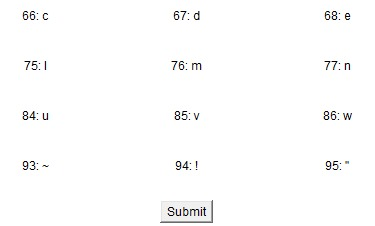
\includegraphics[width=0.3\textwidth]{submit.jpg}
\end{center}
\begin{center}
    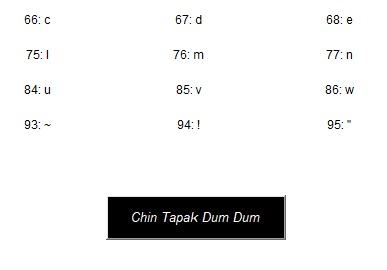
\includegraphics[width=0.3\textwidth]{chin.jpg}
\end{center}

\end{document}
